\newpage
\section{Architecture}
The diagram in Figure \ref{fig:Architecture} shows the overview of the components and tasks of all group-members and their interconnections. The P2000 notifications are collected and passed through a spelling-check. Next, the notifications are indexed in a database. There is also a database of the codes in the notifications with their associated meaning, which is used to process the notifications. The indexed notifications are then processed to be clustered and possible keywords (to link the notifications to news articles or tweets) are extracted. Based on the location and time of the notifications, news articles and tweets are collected. These are also passed through a spelling-check and are indexed in a database afterwards. The news articles and tweets are then clustered and combined with keywords from the clustered notifications and analyzed to find associations. These associations can then be shown to the user as a single incident that occurred. Also the P2000 notifications, news articles and tweets are classified so the user may search for specific kinds of incidents. 

\begin{figure}[h!]
  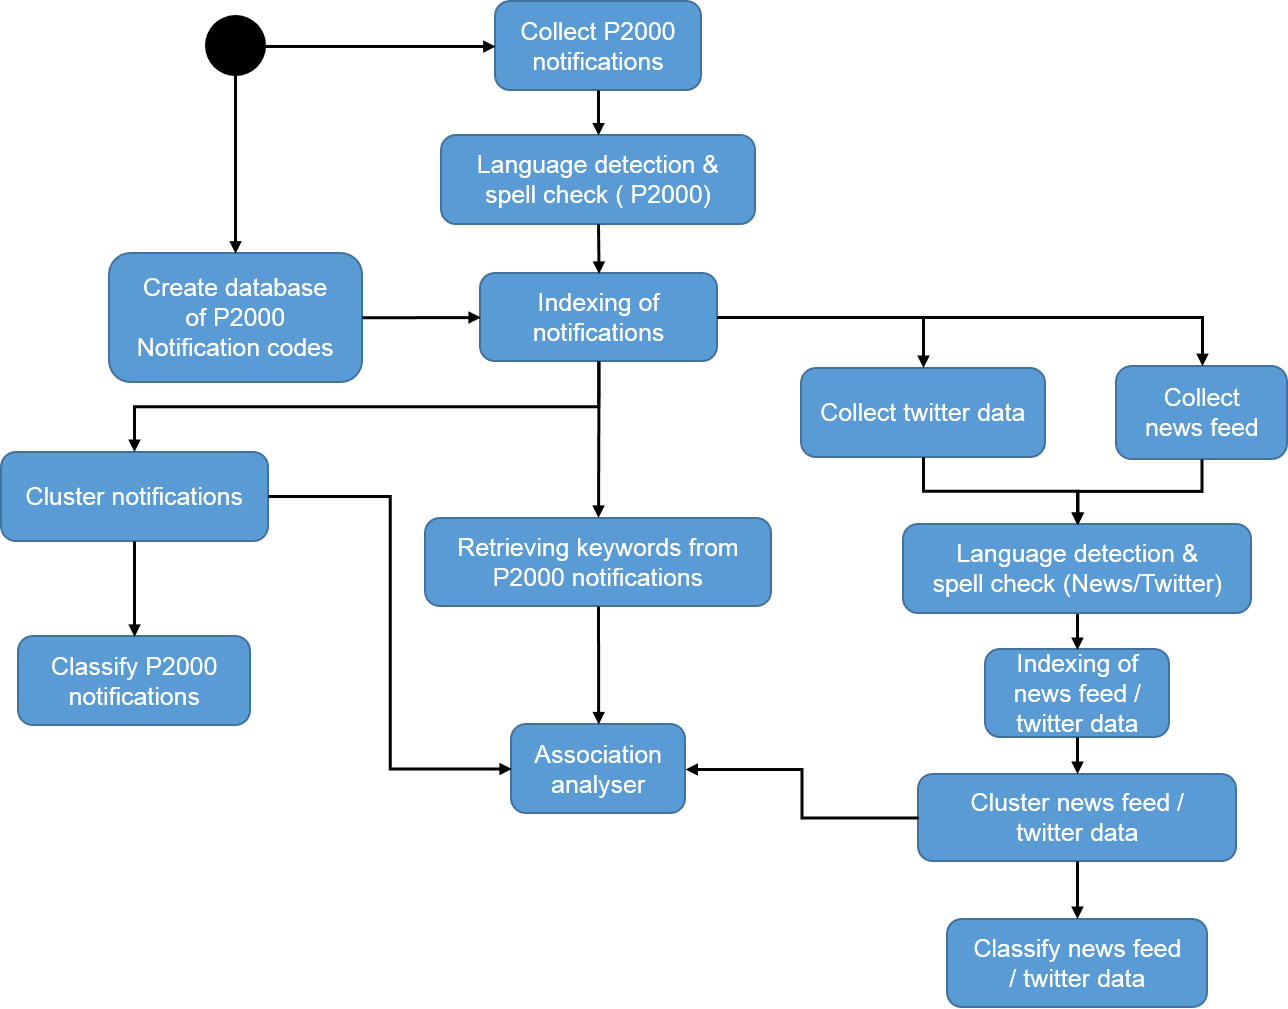
\includegraphics[width=1.0\textwidth]{Architecture.png}
  \caption{Program architecture}
  \label{fig:Architecture}
\end{figure}